\section{Methodology}\label{sec-methodology}

In this paper, a technology developed by Yandex in 2021 that translates
a live stream from English, Spanish, French, Italian, German, or Chinese
into Russian has been used. The translation of a live stream is a
challenging task that has been addressed by the development of a novel
technique based on neural networks. Our study is devoted to the
evaluation of this new technique and focuses on its ability to preserve
the subtleties of semantic meaning and cultural connotations inherent in
phraseological expressions in different linguistic contexts. Although
our study does not address the technical details underlying this tool,
we address these issues as they may help to inform translation. This
technology incorporates advanced machine learning algorithms to enable
the instantaneous translation of language during audiovisual broadcasts.
In essence, this algorithm comprises five fundamental steps, each
executed by a distinct neural network model.

Initially, the audio stream is captured and transcribed into plain text
using automatic speech recognition. The video may contain extraneous
sounds such as noise and music, people may speak with different accents,
speeds and diction, and there may be many speakers, so the technology
must ensure that context and coherence are maintained during the
translation process. Therefore, the algorithm takes a sequence of audio
chunks as input, extracts acoustic features, and passes them into the
neural network. The neural network in turn produces a set of word
sequences from which the language model selects the most plausible
hypothesis.

Subsequently, a machine translation model is employed to translate the
text into the desired target language. There are several problems here:
if you translate word-by-word or phrase-by-phrase, the quality will
suffer, and if you wait for a long pause to guarantee the end of a
sentence, there will be a long delay. So, the technology groups words
into sentences without losing meaning or making sentences too long. For
correct translation at this stage, it is also necessary to determine the
gender of the speaker to determine to whom a particular line belongs and
to reproduce the voice correctly. After selecting individual sentences
and lines, the translation is performed, for which Yandex uses its own
translator.

Once the translation is completed, the translated text is processed
through text-to-speech technology, which converts the written content
into spoken audio. This step ensures that the generated speech sounds
natural and coherent, considering various linguistic features such as
tone, rhythm, and inflection. Additionally, the gender of the speaker,
which was previously identified during the initial stages of the
process, is incorporated into the synthesis to ensure the voice matches
the intended speaker's profile. This level of
customization helps improve the overall quality and authenticity of the
synthesized speech, making it more relatable and contextually
appropriate for the target audience.

Furthermore, the algorithm ensures that the translated speech is
accurately synchronized with the corresponding segments of the video
stream, aligning seamlessly with the visual content, and maintaining
synchronization with the video frames. This process is crucial to ensure
that the audio matches the timing of the speaker's lip movements and
actions in the video. Additionally, the neural network addresses several
challenges in this stage, such as when the speaker delivers a sentence
rapidly, or when the translated sentence is significantly longer than
the original. In these cases, the system must dynamically adjust the
synthesized audio by compressing or shortening it to fit within the
allotted time frame, ensuring smooth and natural speech flow that aligns
with the visual context.

Finally, the translated speech is seamlessly integrated into the live
video stream, replacing the original audio with the newly generated
translated audio. This newly created audio is then encapsulated into an
audio stream, which is embedded directly into the browser interface of
the viewer, allowing them to hear the translated speech while watching
the video in real-time. The technology used for this process is
currently functional exclusively within the Yandex browser, which was
the platform selected for the study. \Cref{fig-01} displays a detailed
screenshot of the Yandex browser interface, clearly highlighting the key
components involved in the translation and audio synchronization
process. It provides a visual representation of how the translated audio
is integrated into the video stream, showing the alignment between the
original video content and the overlaid translated speech. The
screenshot also highlights the user interface elements that facilitate
the viewer's interaction with the translated video, such as volume
controls, language options, and playback features.

\begin{figure}[htpb]
  \centering
  \begin{minipage}{\textwidth}
  \caption{Screenshot of the Yandex browser interface when utilizing 
  the automatic translation features.}
  \label{fig-01}
  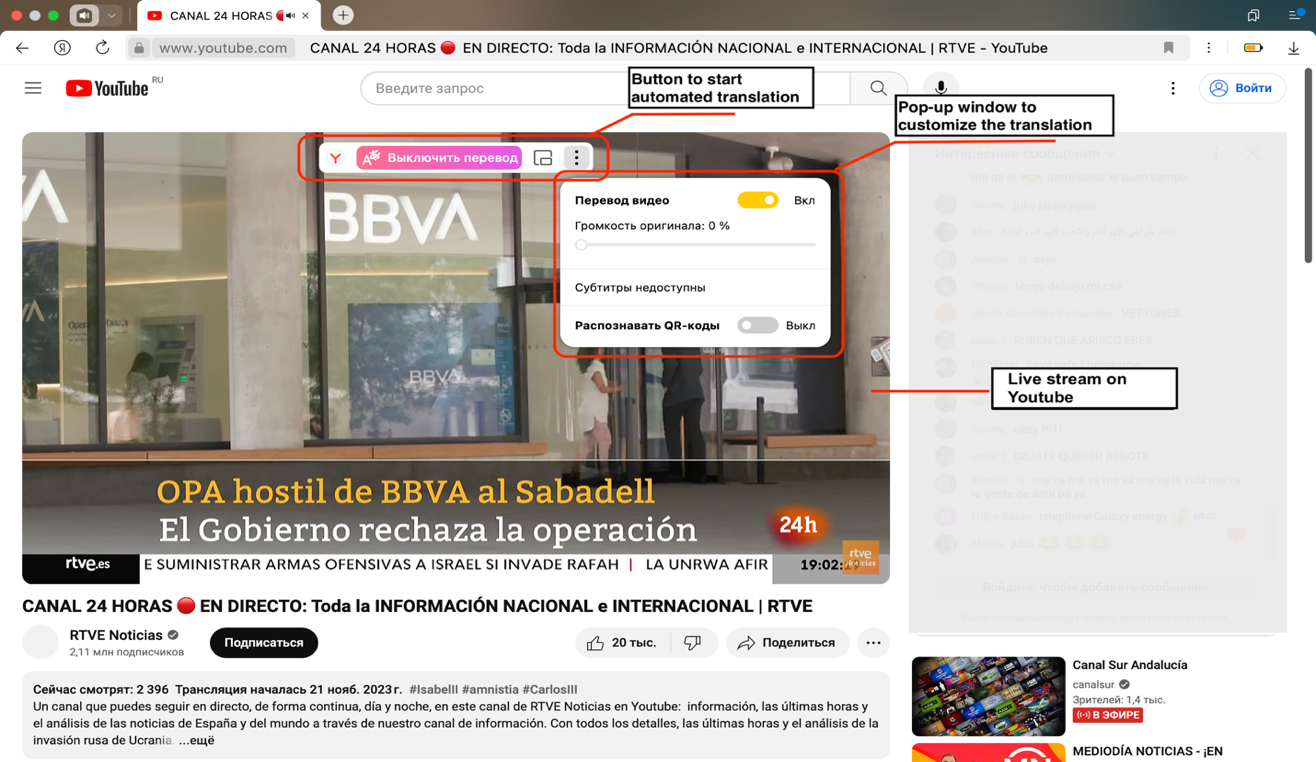
\includegraphics[width=\textwidth]{image1.png}
  \source{Author's own work}
  \end{minipage}
\end{figure}

To enhance the study's transparency and validity, it is
crucial to provide comprehensive details regarding the sample selection,
data collection methods, and the analytical techniques employed. The
live video functionality within the interface is activated via a clearly
visible and easily accessible button, allowing for straightforward
interaction with the system. A notable feature of the translation
process is the 40-50 second temporal delay between the original live
video stream and its translated counterpart in Spanish. This delay, as
derived from a detailed evaluation of the system's operation, is
purposefully incorporated to allow sufficient time for the system to
process the content contextually, which is essential for delivering an
accurate translation in real-time, especially when dealing with live
broadcasts. Such a delay also enables the system to manage the
complexities inherent in real-time translation, such as adjusting for
idiomatic expressions, speech nuances, and varying speaking speeds.

Moreover, the Yandex browser's functionality extends beyond mere passive
translation by allowing users to actively customize their experience.
This includes features like adjusting the volume of the original audio
track, which could be crucial in environments where background noise or
other factors might interfere with the audio quality. Additionally, the
availability of subtitles provides an extra layer of understanding and
flexibility for users, especially in cases where visual cues or context
may not fully suffice to ensure a clear understanding of the translated
content. These customizable features add a significant level of
adaptability to the translation process, catering to various user
preferences and enhancing the overall user experience. Such details are
integral to understanding the technical infrastructure of the study and
ensure its findings can be accurately interpreted and replicated in
future research.

This study employed the Yandex browser and a range of accessible
technological tools to explore the automated translation of live news
streams. The analysis focused on two YouTube channels, ``RTVE Noticias''
and ``Canal Sur Andalucía,'' both of which provide continuous news
coverage. These channels were selected as the primary subjects of
investigation due to their ongoing news broadcasts, providing a robust
sample for examining the translation of live content. The methodology
for the study, as outlined in \Cref{fig-02}, was structured to facilitate a
systematic comparison of the automated translation of phraseological
expressions in real-time news streams.

The approach for comparing the automated translation of phraseological
expressions involved several key stages:

\begin{enumerate}
\def\labelenumi{\arabic{enumi}.}
\item
  \emph{Audio recording:} The first step in the methodology involved
  recording both the original live stream (audio recording \#1) and its
  corresponding translation (audio recording \#2) simultaneously,
  ensuring that both recordings occurred at the same intervals during
  the live broadcast. Two separate devices were used to capture these
  audio recordings concurrently, ensuring precise alignment of the
  original and translated content.
\item
  \emph{Detection of phraseologisms (verbal idioms):} In the second
  stage, instances of phraseologisms, commonly used idiomatic
  expressions, were identified in audio recording \#1, which captured
  the live stream in the original language (Spanish). The identification
  process was carefully carried out to ensure that the expressions
  detected were contextually relevant and representative of the language
  used in the broadcast.
\item
  \emph{Translation matching:} Once the phraseologisms were identified
  in the original audio, the next step involved matching the
  corresponding translations of these expressions in audio recording
  \#2, which was in Russian. This step was crucial for establishing
  whether the automated translation system accurately rendered the
  idiomatic expressions in a culturally appropriate and linguistically
  accurate manner.
\item
  \emph{Comparison and analysis:} The final stage entailed a detailed
  comparison of the accuracy and correctness of the translations. A
  comprehensive comparison table was developed to facilitate this
  process, allowing for a side-by-side evaluation of the original and
  translated expressions. The total duration of the audio recordings in
  both Spanish (the original language) and Russian (the translated
  language) amounted to 243 minutes for each language. These recordings
  were made across different intervals, ranging from 15 to 60 minutes,
  and were captured on multiple occasions throughout the day over four
  non-consecutive days. This sampling strategy was employed to ensure a
  diverse representation of news topics covered during the broadcasts.
  As part of the analysis, 52 verbal idioms were identified and
  thoroughly examined within the context of the live news stream,
  providing insights into the effectiveness of the automated translation
  system in handling phraseological expressions in a dynamic, real-time
  setting.
\end{enumerate}

\begin{figure}[htpb]
  \centering
  \begin{minipage}{\textwidth}
  \caption{General outline of the methodology presented.}
  \label{fig-02}
  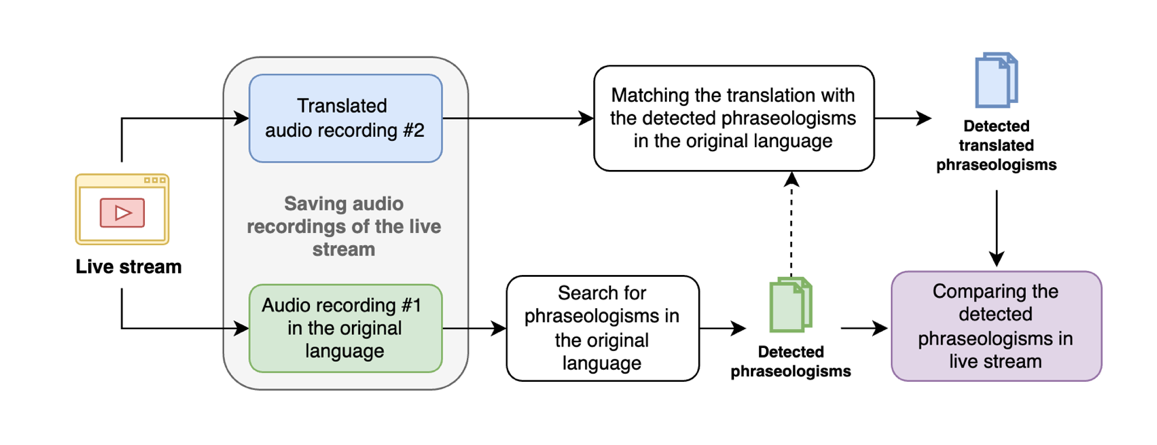
\includegraphics[width=\textwidth]{image2.png}
  \source{Author's own work.}
  \end{minipage}
\end{figure}



